\chapter{Language Implementation}


\section{Data Type}
\subsection{Tokenizer Type}
All tokens are define using the Haskell Lexer Generator Alex.Tokens will be recognized and converted to Haskell data types.For example , a valid variable is comprised with one or more alphabetic characters and digit and the first character must be an alphabetic characters. This rule can be defined as ,
\begin{lstlisting}[language=java]
$digit = 0-9			-- digits
$lowerCase = [a-z]
$alpha = [a-zA-Z]		-- alphabetic characters

tokens :-
  $alpha [$alpha $digit \_ \' \.]* { \s -> TName s }
-- data definition
data Token = 
	TName String |
	TBool Bool  | 
	TInt Int  | 
	...  -- more definition			

\end{lstlisting}

The variable \textbf{var1} will be parse into Haskell data type \textbf{TName "var1"}\\


By using the lexer , all the code will be generated into tokens streams.
\begin{lstlisting}[language=java]
program myProgram ()
{
	var1 = 1;
	result = var1 + "a string";
}
\end{lstlisting}

The following codes show the invocation of the lexer and the returned tokens stream.
\begin{lstlisting}[language=java]
lexer "program myProgram() { var1 = 1; result = var1 + False; return 0; }"
[TProgram,TName "myProgram",TOPB,TCPB,TOCB,TName "var1",TAssign,TInt 1,TSC,TName "result",TAssign,TName "var1",TPlus,TBool False,TSC,TReturn,TInt 0,TSC,TCCB]
\end{lstlisting}



\subsection{Parser internal data type}
The Parser internal data type typically represents a parse tree.To represent a generic expression,we can define data type as follow,

\begin{hcode}
data GenericExp  =
		     Var String 
		   | Int Int
		   | Double Double
		   | Plus GenericExp GenericExp		   
		   | ListIndex String [GenericExp]
		   | Brack GenericExp  deriving 
		   ... -- more definition
\end{hcode}


The following code 
\begin{lstlisting}[language=java]
( a +1 )  /=  3
myArray[ 1+1,2] 
\end{lstlisting}

are parsed into Haskell data structure,

\begin{hcode}
NotEq  (Brack ( Plus (Var "a") (Int 1)))  (Int 3)
ListIndex "myIndex" [ Plus (Int 1) (Int 1) , Int 2 ] 
\end{hcode}


\begin{figure}[H]
  \centering
	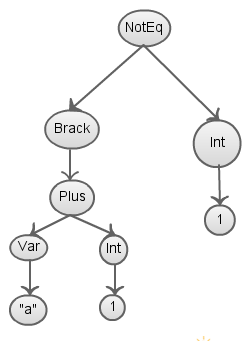
\includegraphics[width=0.40\textwidth]{pic/c6/parse_tree_1.png}
	\caption{Diagram illustrating a parse tree of a generic expression}
\end{figure}


In Haskell,a parse tree data structure that support polymorphic list can be defined using recursive data type as follow, 
\begin{hcode}
data List = ListGenericExp GenericExp
			| ListList [List] deriving (Show,Eq,Read)  
\end{hcode}


A polymorphic list,
\begin{lstlisting}[language=java]
 [1,2,["string",2,3]];
\end{lstlisting}

Can be represent in Haskell data type.

\begin{hcode}
ListList  [ListGenericExp (Int 1),ListGenericExp (Int 2),
	ListList [ListGenericExp String "string",
		ListGenericExp (Int 2),ListGenericExp (Int 3)]] 
\end{hcode}



\begin{figure}[H]
  \centering
	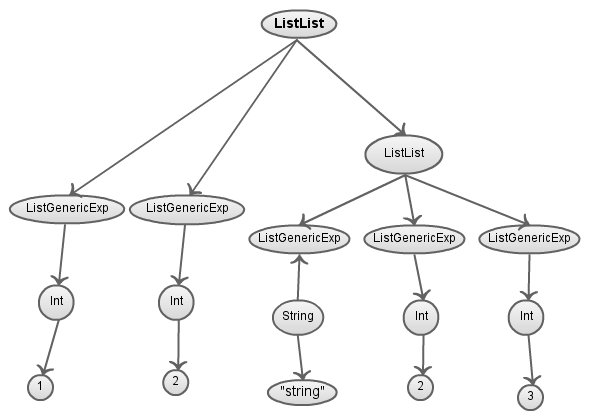
\includegraphics[width=0.90\textwidth]{pic/c6/parse_tree_2.png}
	\caption{Diagram illustrating a parse tree of a list expression}
\end{figure}


\subsection{Interpreter internal data type}

\section{Statement Interpreter}

\section{Symbol Table and Parse Tree}


\section{Generic Expression Interpreter}

\subsection{Function Invocation}
